\section{Ejercicios 1 y 2}
Para ver gráficamente el comportamiento del scheduler FCFS, creamos un lote de tareas que tenía uso intensivo de CPU, y dos tareas que sólo ejecutan llamadas bloqueantes (una con muchas llamadas cortas y una con pocas más largas).
\begin{figure}[h]
  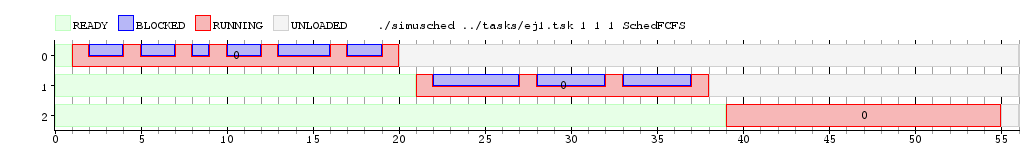
\includegraphics[width=\textwidth]{ej1-2/figs/ej1-1core.png}
  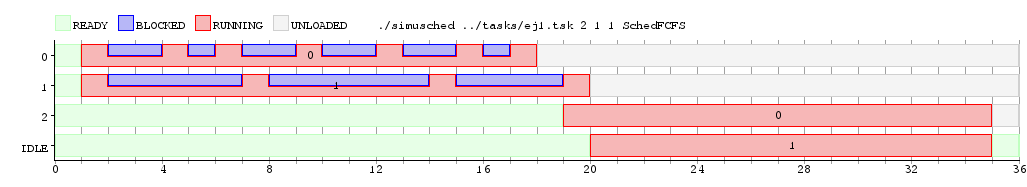
\includegraphics[width=\textwidth]{ej1-2/figs/ej1-2core.png}
  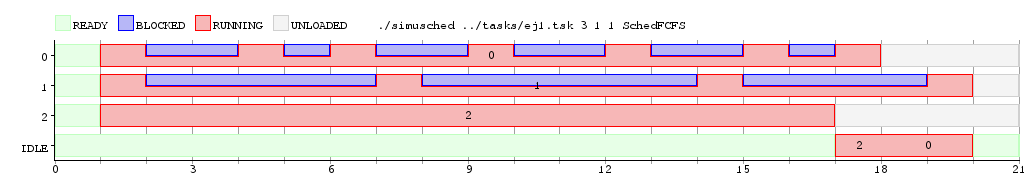
\includegraphics[width=\textwidth]{ej1-2/figs/ej1-3core.png}
  \caption{Diagramas de Gantt para la simulación con 1, 2 y 3 núcleos respectivamente.}
\end{figure}

Los procesos se ejecutan siempre hasta que se terminan, por lo tanto permanecen ejecutando aún estando bloqueados.
